\chapter{Classical cluster algebras}
Mostly use \cite{FominWilliams2021IntroductionCA_1-3} as reference together with
Geoffrey's notes.

\section{Cluster algebras from quivers}

This first section serves as an introduction to cluster algebras. We will first look at
some examples of integer sequences arising from number theory or from combinatorial
data. In these examples, a few recurring observations will occur. These observations
will be explained by viewing each of the examples under the lens of cluster algebra
theory. We do not yet provide the most general definition of a cluster algebra, which
will instead be done in \cref{sec:ice_quivers_and_coefficients}. Instead, we focus on
the simplest case of a cluster algebra associated to a quiver. This case is easier to
grasp, and allows understanding the general concepts without getting distracted by
technical details.

\subsection{Combinatorial integer sequences}\label{sec:integer_sequences}

Let us start by looking at some integer sequences coming from number theory or
combinatorial data. Along the way we observe some interesting patterns which will be
explained by viewing these sequences as arising from a cluster algebra. \medskip

\begin{example}\label{exmp:markov_sequence}
	Consider the sequence given by the recurrence relation
	\begin{equation*}
		x_{n+3} = \frac{x_{n+1}^2 + x_{n+2}^2}{x_n},
	\end{equation*}
	with initial conditions $x_0 = x_1 = x_2 = 1$. Computing the first few terms gives
	\begin{equation*}
		1,1,1,2,5,29,433,37666,48928105,\dots
	\end{equation*}
	%
	Even though the recurrence relation involves a fraction, all the terms of the sequence
	are positive integers. We will explain this later, as a consequence of a more general
	fact about cluster algebras. Another way to observe this is as follows. For each $n \in
		\bbZ_{\geq0}$, the triple $(x_n, x_{n+1}, x_{n+2})$ satisfies the equation
	\begin{equation}\label{eq:markov_diophantine}
		x_n^2 + x_{n+1}^2 + x_{n+2}^2 = 3 x_n x_{n+1}x_{n+2},
	\end{equation}
	known as the \emph{Markov equation}\index{Markov!equation}\footnote{It is named after Andrey Markov. This is the same mathematician after whom Markov chains are named.}. The case $n = 0$ is clear. Then, by induction, we have
	\begin{equation}\label{eq:markov_mutation_simplified}
		x_{n+3} = \frac{x_{n+1}^2 + x_{n+2}^2}{x_n} = \frac{3 x_n x_{n+1}x_{n+2} - x_n^2}{x_n} = 3 x_{n+1} x_{n+2} - x_n,
	\end{equation}
	so that
	\begin{align*}
		x_{n+3}^2 + x_{n+2}^2 + x_{n+1}^2
		 & = (3 x_{n+1}x_{n+2} - x_n)^2 + x_{n+1}^2 + x_{n+2}^2                            \\
		 & = 9 x_{n+1}^2 x_{n+2}^2 - 6 x_{n+1} x_{n+2} x_n + x_n^2 + x_{n+1}^2 + x_{n+2}^2 \\
		 & = 9 x_{n+1}^2 x_{n+2}^2 - 6 x_n x_{n+1} x_{n+2} + 3 x_n x_{n+1} x_{n+2}         \\
		 & = 9 x_{n+1}^2 x_{n+2}^2 - 3 x_n x_{n+1} x_{n+2}                                 \\
		 & = 3 ( x_{n+1} x_{n+2}-  x_n) x_{n+1} x_{n+2}                                    \\
		 & = 3 x_{n+3} x_{n+1} x_{n+2}.
	\end{align*}
	%
	The intermediate result, \cref{eq:markov_mutation_simplified}, also immediately implies
	that all the terms in the sequence are integers. That they are positive follows from
	the recurrence relation itself.
\end{example}

\begin{example}\label{exmp:somos4}

	Let $a_n$ be the sequence defined through the recurrence relation
	\begin{equation}
		\label{eq:somos_4}
		a_{n+4} = \frac{a_{n+3}a_{n+1}+ a_{n+2}^2}{a_n}
	\end{equation}
	%
	with initial conditions $a_0 = a_1 = a_2 = a_3 = 1$. This sequence is known as the
	\emph{Somos-4}\index{Somos-4 sequence} sequence, named after its inventor, Michael
	Somos. It can be seen as a slight generalization of the sequence from
	\cref{exmp:markov_sequence}. Computing the first few terms of the sequence, we find:
	\begin{align*}
		 & \begin{aligned}
			   a_4 & = \frac{1 \cdot 1 + 1^2}{1} = 2                   \\
			   a_5 & = \frac{2 \cdot 1 + 1^2}{1} = 3                   \\
			   a_6 & = \frac{3 \cdot 1 + 2^2}{1} = 7                   \\
			   a_7 & = \frac{7 \cdot 2 + 3^2}{2} = 23                  \\
			   a_8 & = \frac{23 \cdot 3 + 7^2}{2} = \frac{118}{2} = 59 \\
		   \end{aligned}
		 &
		\begin{aligned}
			a_9    & = \frac{59 \cdot 7 + 23^2}{3} = \frac{942}{3} = 314                       \\
			a_{10} & = \frac{314 \cdot 23 + 59^2}{7} = \frac{10703}{7} = 1529                  \\
			a_{11} & = \frac{1529 \cdot 59 + 314^2}{23} = \frac{188807}{23} = 8209             \\
			a_{12} & = \frac{8209 \cdot 314 + 1529^2}{59} = \frac{4915467}{59} = 83313         \\
			a_{13} & = \frac{83313 \cdot 1529 + 8209^2}{314} = \frac{194773258}{314} = 620297.
		\end{aligned}
	\end{align*}
	%
	Just like in the previous example, there is no reason, a priori, to assume that all the
	elements of the sequence would be integers. However, somewhat remarkably, the
	denominators seem to always cancel out perfectly. Viewing this sequence through the
	cluster algebra framework, it will follow immediately that all the terms are indeed
	integers, as a corollary of the \emph{Laurent phenomenon}\index{Laurent!-phenomenon}.
\end{example}

\begin{example}\label{exmp:frieze_patterns}

	The next family of integer sequences comes from \emph{$\SL_2(\bbZ)$-frieze
		patterns}\footnote{The name ``frieze pattern'' comes from architecture, where it refers
		to a horizontal strip, often found just below the roofline, which is decorated with
		patterns.}\index{frieze pattern}\index{SL 2 Z@$\SL_2(\bbZ)$}. The idea of a frieze
	pattern is best explained through an example (\cite{Coxeter1971FriezePatterns}). Take
	for example the following pattern:
	\begin{equation*}
		\dots\quad
		\begin{tikzcd}[
				sep = 0.2em, cramped,
			]
			&0&&0&&0&&0&&0&&0&&0&&0&&0&&0&&0\\
			1&&1&&1&&1&&1&&1&&1&&1&&1&&1&&1\\
			&1&&2&&2&&3&&1&&2&&4&&1&&2&&2&&3\\
			3&&1&&3&&5&&2&&1&&7&&3&&1&&3&&5\\
			&2&&1&&7&&3&&1&&3&&5&&2&&1&&7&&3\\
			3&&1&&2&&4&&1&&2&&2&&3&&1&&2&&4\\
			&1&&1&&1&&1&&1&&1&&1&&1&&1&&1&&1\\
			0&&0&&0&&0&&0&&0&&0&&0&&0&&0&&0
		\end{tikzcd}
		\quad
		\dots
	\end{equation*}
	The defining property is that the $2 \times 2$ diamonds
	\begin{equation*}
		\begin{matrix}
			  & b &   \\
			a &   & d \\
			  & c &
		\end{matrix}
	\end{equation*}
	formed by adjacent elements, can be seen as an element of $\SL_2 (\bbZ)$, i.e., $ad - bc = 1$. Other than the bounding rows of ones and zeros, there is no additional requirement. In what follows we will omit the irrelevant row of zeros.

	One could ask if it is always possible to construct such a pattern for any number of
	rows. If so, one might be interested in knowing how many such patterns there are.
	Furthermore, one might notice that the pattern is periodic, repeating every 7 columns.
	In fact, the pattern even has ``half-periodicity'' where the marked triangle undergoes
	a translation and reflection.
	\begin{equation*}
		\dots\quad
		\begin{tikzcd}[
				sep = 0.2em, cramped,
				execute at end picture = {
						\draw[blue, dashed, rounded corners]
						($(\tikzcdmatrixname-1-1.north west) + (-0.3, 0.05)$) -- ($(\tikzcdmatrixname-1-11.north east)+ (0.3, 0.05)$)--($(\tikzcdmatrixname-6-6.south) + (0,-0.05)$) -- cycle;
						\draw[red, dashed, rounded corners]
						($(\tikzcdmatrixname-6-8.south west) + (-0.3, -0.05)$) -- ($(\tikzcdmatrixname-6-18.south east)+ (0.3, -0.05)$)--($(\tikzcdmatrixname-1-13.north) + (0,0.05)$) -- cycle;
					}
			]
			1&&1&&1&&1&&1&&1&&1&&1&&1&&1&&1\\
			&1&&2&&2&&3&&1&&2&&4&&1&&2&&2&&3\\
			3&&1&&3&&5&&2&&1&&7&&3&&1&&3&&5\\
			&2&&1&&7&&3&&1&&3&&5&&2&&1&&7&&3\\
			3&&1&&2&&4&&1&&2&&2&&3&&1&&2&&4\\
			&1&&1&&1&&1&&1&&1&&1&&1&&1&&1&&1\\
		\end{tikzcd}
		\quad
		\dots
	\end{equation*}

	To make such a pattern, we start with the observation that the rest of the pattern is
	completely determined by a lattice path from top to bottom. Indeed, using the
	$\SL_2(\bbZ)$ rule, one can fill in the rest of the pattern. For example, say we
	started with the following partially filled in pattern:
	\begin{equation*}
		\dots\quad
		\begin{tikzcd}[
				sep = 0.2em, cramped,
			]
			1&&1&&1&&1&&1&&1&&1\\
			&a\\
			b\\
			&1&&1&&1&&1&&1&&1\\
		\end{tikzcd}
		\quad
		\dots
	\end{equation*}
	then the rest has to be filled out as follows
	\begin{equation*}
		\dots\quad
		\begin{tikzcd}[
				sep = 0.2em, cramped,
			]
			1&&1&&1&&1&&1&&1&&1\\
			&a&& \frac{1+a+b}{ab} && b && \frac{1+a}{b} && \frac{1+b}{a} && a\\
			b&& \frac{1+a}{b} &&  \frac{1+b}{a} && a && \frac{1+a+b}{ab} && b\\
			&1&&1&&1&&1&&1&&1\\
		\end{tikzcd}
		\quad
		\dots
	\end{equation*}
	%
	Since all the denominators are monomials in $a$ and $b$, it follows that when $a = b =
		1$, all the elements will be integers, as required.

	It seems that we somehow got lucky in this case. There is again, a priori, no reason to
	assume that for any number of rows, we will always be able to choose the initial
	integers such that all the fractions simplify. The fact that this is possible, follows
	again from the ``Laurent phenomenon''\index{Laurent!-phenomenon}, on which we can now
	shed a bit more light. Let $a_1, a_2, \dots, a_n$ be the initial integers chosen on the
	lattice path. Then, in this context, the Laurent phenomenon states that all the other
	elements of the frieze pattern can be written as Laurent
	polynomials\index{Laurent!-polynomial} in $a_1 , \dots, a_n$ with coefficients in
	$\bbZ$, i.e., as an element of $\bbZ [a_1 ^\pm, \dots, a_n^\pm]$. So, any lattice path
	from top to bottom consisting of only ones, will yield a frieze pattern. This already
	proves the existence of such frieze patterns for any number of rows. We will return to
	the other questions in \cref{sec:sequences_revisited}.
\end{example}

The last example will be based on the following theorem from Euclidean geometry.
\begin{theorem}[Ptolomy's Theorem]\label{thm:ptolomy}

	Let $A,B,C,D$ be distinct points on a circle, in cyclic order (\cref{fig:ptolomy}).
	These determine vertices of a quadrilateral, where the side, and diagonal lengths
	satisfy the following rule:
	\begin{equation*}
		|AC| \cdot |BD| = |AB|\cdot |CD| + |AD| \cdot |BC|.
	\end{equation*}
\end{theorem}

\begin{figure}
	\centering

	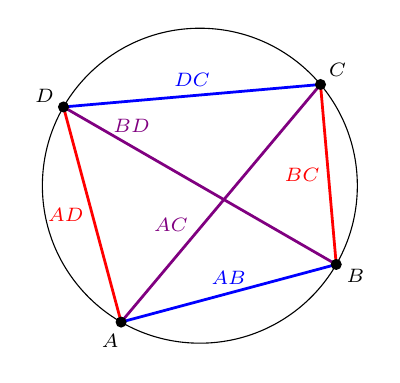
\begin{tikzpicture}
		\coordinate (center) at (0,0);
		\def\radius{2cm}
		\draw (center) circle[radius=\radius];

		% points on the circle
		\path (center) ++(-120:\radius) coordinate (A);
		\path (center) ++(-30:\radius) coordinate (B);
		\path (center) ++(40:\radius) coordinate (C);
		\path (center) ++(150:\radius) coordinate (D);

		\begin{scriptsize}
			% Chords
			\draw[color=red, line width=1pt] (A) -- node[left] {$AD$} (D);
			\draw[color=red, line width=1pt] (B) -- node[left] {$BC$} (C);
			\draw[color=blue, line width=1pt] (A) -- node[above] {$AB$} (B);
			\draw[color=blue, line width=1pt] (D) -- node[above] {$DC$} (C);
			\draw[color=violet, line width=1pt] (A) -- node[above=8pt, near start] {$AC$} (C);
			\draw[color=violet, line width=1pt] (D) -- node[above=2pt, near start] {$BD$} (B);

			% Draw the points over the chords
			\fill[black] (A) circle[radius=2pt] ++(-120:1em) node {$A$};
			\fill[black] (B) circle[radius=2pt] ++(-30:1em) node {$B$};
			\fill[black] (C) circle[radius=2pt] ++(40:1em) node {$C$};
			\fill[black] (D) circle[radius=2pt] ++(150:1em) node {$D$};

		\end{scriptsize}
	\end{tikzpicture}
	\caption{Ptolomy's theorem:
	${\color{violet} |AC| \cdot |BD|}
		= {\color{red} |AD|\cdot |BC|} + {\color{blue} |AB| \cdot |CD|}$.}
	\label{fig:ptolomy}
\end{figure}

\begin{example}\label{exmp:triangulations}

	Note that \cref{thm:ptolomy} allows one to compute the length of one of the diagonals
	in terms of the other, given the side lengths. We will now apply this to triangulations
	of polygons.

	Let $1, 2, \dots, n$ denote $n$ points on a circle, arranged in cyclic order. By
	connecting these points through sides $P_{i, i+1}$, where the indices are taken modulo
	$n$, we obtain a polygon with $n$-sides. A triangulation\index{triangulations!of
		polygons}, $T$, is a choice of $(n-3)$ non-crossing diagonals. This results in a
	partitioning of the polygon in $n-2$ triangles. We will see triangulations in much more
	detail in \cref{sec:triangulations_of_surfaces}, and will therefore keep things brief
	here. For now, it is enough to understand things visually (cf.
	\cref{fig:hexagon_triangulations}).
	\begin{figure}[ht]
		\centering

		\begin{tikzpicture}
			\node[name=h, shape=regular polygon, draw, regular polygon sides = 6, minimum size = 1.5cm]{};
			\draw[] (h.corner 1) -- (h.corner 3);
			\draw[] (h.corner 1) -- (h.corner 4);
			\draw[] (h.corner 1) -- (h.corner 5);
		\end{tikzpicture}
		\begin{tikzpicture}
			\node[name=h, shape=regular polygon, draw, regular polygon sides = 6, minimum size = 1.5cm]{};
			\draw[] (h.corner 2) -- (h.corner 5);
			\draw[] (h.corner 2) -- (h.corner 4);
			\draw[] (h.corner 1) -- (h.corner 5);
		\end{tikzpicture}
		\begin{tikzpicture}
			\node[name=h, shape=regular polygon, draw, regular polygon sides = 6, minimum size = 1.5cm]{};
			\draw[] (h.corner 1) -- (h.corner 3);
			\draw[] (h.corner 3) -- (h.corner 5);
			\draw[] (h.corner 1) -- (h.corner 5);
		\end{tikzpicture}
		\caption{The triangulations of a regular hexagon up to rotation.}
		\label{fig:hexagon_triangulations}
	\end{figure}

	Starting from a triangulation, $T$, we obtain a new triangulation, $T'$, by
	``flipping'' a diagonal. Any diagonal in a triangulation lies on precisely 2 triangles.
	These two triangles form a quadrilateral. To flip the diagonal, you replace it with the
	other diagonal of that quadrilateral. Again, this is most easily seen visually:
	\begin{equation*}
		\begin{tikzpicture}[baseline]
			\node[name=h, shape=regular polygon, draw, regular polygon sides = 6, minimum size = 1.5cm]{};
			\draw[] (h.corner 1) -- (h.corner 3);
			\draw[dashed] (h.corner 1) -- (h.corner 4);
			\draw[] (h.corner 1) -- (h.corner 5);
		\end{tikzpicture}
		\quad \leadsto \quad
		\begin{tikzpicture}[baseline]
			\node[name=h, shape=regular polygon, draw, regular polygon sides = 6, minimum size = 1.5cm]{};
			\draw[] (h.corner 1) -- (h.corner 3);
			\draw[dashed] (h.corner 3) -- (h.corner 5);
			\draw[] (h.corner 1) -- (h.corner 5);
		\end{tikzpicture}
	\end{equation*}
	%
	Using Ptolomy's theorem, the length of the new diagonal can be computed given that we
	knew the lengths of all the edges in the previous triangulation. We now ignore
	Euclidean geometry, and just use Ptolomy's theorem as a recurrence relation to
	construct a collection of numbers as follows. Pick a triangulation and set all the edge
	lengths equal to one. Then at each step, choose a diagonal in the triangulation and
	flip it. Compute its edge length using Ptolomy's theorem. This is the next number in
	the collection. For example, we could obtain a sequence starting like this (we omit the
	ones on the sides):
	\begin{equation*}
		\begin{tikzpicture}[baseline]
			\node[name=h, shape=regular polygon, draw, regular polygon sides = 6, minimum size = 1.5cm]{};
			\draw[] (h.corner 1) -- node[fill=white, font=\footnotesize] {1} (h.corner 3);
			\draw[] (h.corner 1) -- node[fill=white, font=\footnotesize] {1} (h.corner 4);
			\draw[] (h.corner 1) -- node[fill=white, font=\footnotesize] {1} (h.corner 5);
		\end{tikzpicture}
		\leadsto
		\begin{tikzpicture}[baseline]
			\node[name=h, shape=regular polygon, draw, regular polygon sides = 6, minimum size = 1.5cm]{};
			\draw[] (h.corner 1) -- node[fill=white, font=\footnotesize] {1} (h.corner 3);
			\draw[dashed] (h.corner 3) -- node[fill=white, font=\footnotesize] {2} (h.corner 5);
			\draw[] (h.corner 1) -- node[fill=white, font=\footnotesize] {1} (h.corner 5);
		\end{tikzpicture}
		\leadsto
		\begin{tikzpicture}[baseline]
			\node[name=h, shape=regular polygon, draw, regular polygon sides = 6, minimum size = 1.5cm]{};
			\draw[dashed] (h.corner 2) -- node[fill=white, font=\footnotesize] {3} (h.corner 5);
			\draw[] (h.corner 3) -- node[fill=white, font=\footnotesize] {2} (h.corner 5);
			\draw[] (h.corner 1) -- node[fill=white, font=\footnotesize] {1} (h.corner 5);
		\end{tikzpicture}
		\leadsto
		\begin{tikzpicture}[baseline]
			\node[name=h, shape=regular polygon, draw, regular polygon sides = 6, minimum size = 1.5cm]{};
			\draw[] (h.corner 2) -- node[fill=white, font=\footnotesize] {3} (h.corner 5);
			\draw[] (h.corner 3) -- node[fill=white, font=\footnotesize] {2} (h.corner 5);
			\draw[dashed] (h.corner 2) -- node[fill=white, font=\footnotesize] {4} (h.corner 6);
		\end{tikzpicture}
		\leadsto
		\begin{tikzpicture}[baseline]
			\node[name=h, shape=regular polygon, draw, regular polygon sides = 6, minimum size = 1.5cm]{};
			\draw[dashed] (h.corner 3) -- node[fill=white, font=\footnotesize] {3} (h.corner 6);
			\draw[] (h.corner 3) -- node[fill=white, font=\footnotesize] {2} (h.corner 5);
			\draw[] (h.corner 2) -- node[fill=white, font=\footnotesize] {4} (h.corner 6);
		\end{tikzpicture}
		\leadsto
		\begin{tikzpicture}[baseline]
			\node[name=h, shape=regular polygon, draw, regular polygon sides = 6, minimum size = 1.5cm]{};
			\draw[] (h.corner 3) -- node[fill=white, font=\footnotesize] {3} (h.corner 6);
			\draw[] (h.corner 3) -- node[fill=white, font=\footnotesize] {2} (h.corner 5);
			\draw[dashed] (h.corner 3) -- node[fill=white, font=\footnotesize] {1} (h.corner 1);
		\end{tikzpicture}
		\leadsto \cdots
	\end{equation*}
	%
	Once again, we observe that we only obtain integers. Furthermore, there seems to be a
	limit to which integers we can obtain this way. This hints at a hidden periodicity. The
	Laurent phenomenon offers an explanation for why we only obtain integers: the lengths
	of the diagonals are Laurent polynomials in the originally chosen lengths.
\end{example}

There are many more examples like the three that we just gave. One can look at wiring
diagrams, generalized Somos sequences, knight recurrence, the Gale-Robinson sequence,
etc. As the focus of this thesis is not on number theory, we refrain from delving
deeper into this interesting world. We refer interested readers to \cite[Chapter
	3.4]{FominWilliams2021IntroductionCA_1-3} and \cite{FominZelevinsky2002Laurent}.

\subsection{Quivers, seeds and mutations}\label{sec:quivers_seeds_mutations}

In the examples from \cref{sec:integer_sequences} we made a couple of observations. In
each case, the sequence consisted of positive integers, something which was not so
obvious from the initial definitions. For
\cref{exmp:frieze_patterns,exmp:triangulations}, we also found some form of finiteness
and periodicity. There are some more subtle similarities, which will be explained in
detail in \cref{sec:sequences_revisited}. Before that, we must introduce the notion of
a cluster algebra. These can be constructed from a quiver, as we now explain.

\begin{definition}[Quivers]

	A \emph{quiver}\index{quiver} is a finite directed (multi)-graph with no 1-cycles
	(vertex connected to itself) or 2-cycles (two vertices connected by a pair of opposite
	arrows) (cf. \cref{fig:quivers}). For a quiver $Q$, we will denote the set of vertices
	with $Q_0$\index{Q 0@$Q_0$}.
\end{definition}

\begin{figure}[ht!]
	\centering
	\begin{equation*}
		\begin{tikzcd}
			&\bullet \arrow[loop] \arrow[r] &\bullet \\
			\bullet \rar & \bullet \arrow[r, bend left] & \bullet \arrow[l, bend left]
		\end{tikzcd}
		\hspace{2cm}
		\begin{tikzcd}[row sep=small]
			&&& \bullet \\
			\bullet \ar[rrrd, bend right]\rar &\bullet  \rar[leftarrow] &\bullet \ar[ru, shift left] \ar[ru, shift right] \ar[rd] \\
			&&& \bullet\\
			\\
			\bullet \ar[rr] && \bullet \ar[ld]\\
			& \bullet \ar[lu]
		\end{tikzcd}
	\end{equation*}
	\caption{The graphs on the left are not quivers, the graphs on the right are.}
	\label{fig:quivers}
\end{figure}

Let us now fix some notation for what follows. Write $[a,b] = \{a, a + 1, \dots, b\}$
for integers $a,b \in \bbZ$, where $[a,b] = \emptyset$ if $a > b$. Fix an integer $N
	\in \bbZ_{\geq 0}$. Finally, let $\mcF = \bbQ (Y_1, \dots, Y_N)$ be the \emph{field of
	rational functions}\index{rational function field} over $\bbQ$, in $N$ variables. Thus,
$\mcF$ consists of fractions $P/Q$ where $P, Q\in \bbQ[Y_1, \dots, Y_N]$ are
polynomials in the variables $Y_1, \dots, Y_N$, and $Q$ is non-zero.

\begin{definition}
	We call a pair $(Q, \bx)$ a \emph{labeled seed}\index{seed!labeled} if
	\begin{enumerate}
		\item $Q$ is a quiver with vertices $Q_0 = [1, N]$.
		\item $\bx = \{x_1, \dots, x_N\}$ is a \emph{free generating set} of $\mcF$. That is, $\bx$ is a set of $N$ algebraically independent elements that generate $\mcF$.
	\end{enumerate}
	The set $\bx$ will be referred to as the \emph{cluster}\index{cluster}. The elements of $\bx$ will be called \emph{cluster variables}\index{cluster!variables}.
\end{definition}
%
One can also talk about \emph{unlabeled seeds}\index{seed!unlabeled}. An unlabeled seed
is an equivalence class of labeled seeds which are equal up to a simultaneous
re-indexing of the quiver vertices and the cluster variables. We will not need
unlabeled seeds as much, and will hence adopt the following convention.
\begin{convention}
	From now on, when we say \emph{seed}, we will always mean a labeled seed.
\end{convention}

Just like in nature, a seed on it own is not so interesting. We are interested in what
one can obtain from the seed. From a given seed, we can make another seed through a
process known as \emph{seed mutation}\index{seed!mutation}.
\begin{definition}

	Let $k \in \ex$ be an exchangeable vertex of the quiver $Q$. We define the
	\emph{mutation in direction $k$} of the seed $(Q, \bx)$ to be the seed $\mu_k(Q, \bx)
		\defeq (Q', \bx') = (\mu_k(Q), \mu_k(\bx))$\index{mu k@$\mu_k$}, where
	\begin{enumerate}
		\item $Q'_0 \defeq Q_0$.
		\item For every pair of vertices $i,j$ with $s$ arrows $i \to k$ and $t$ arrows $k \to j$ we
		      ``collapse'' these arrows into $s\cdot t$ arrows $i \to j$, cancelling pairwise with
		      any arrows $j \to i$.
		      \begin{equation*}
			      \begin{tikzcd}[column sep=small]
				      i \ar[rr, "r"] \ar[rd, "s"] && j \\
				      & k \ar[ur, "t"]
			      \end{tikzcd}
			      \quad \begin{tikzcd}
				      \; \rar[rightsquigarrow, "\mu_k"]& \;
			      \end{tikzcd}\quad
			      \begin{tikzcd}[column sep=small]
				      i \ar[rr, "r + st"] \ar[rd,leftarrow, "s"] && j \\
				      & k \ar[ur, leftarrow, "t"]
			      \end{tikzcd}
		      \end{equation*}
		      Here we take $r$ to be negative, if the arrows actually point the other way, as the path $i \to k \to j$.
		      If $i,j$ are both frozen, then we ignore this step.
		\item All arrows in $Q$ starting or ending in $k$ get their orientation flipped.
		\item $\bx' = \{x_1', \dots, x_N'\}$, where $x_i' = x_i$ for $i \neq k$, and $x'_k$
		      is given by the \emph{exchange relation}\index{exchange relation}
		      \begin{equation}\label{eq:exchange_relation_quiver}
			      x'_k \defeq \frac{1}{x_k} \left(\prod_{i \to k} x_i + \prod_{k \to j} x_j\right),
		      \end{equation}
		      where we take the product equal to 1 if $\{i \to k\} = \emptyset$ or $\{k \to j\} = \emptyset$.
	\end{enumerate}
\end{definition}

Let us first look at an example involving only the mutation of the quiver.
\begin{example}
	We mutate the given quiver at vertex 2:
	\begin{equation*}
		\begin{tikzcd}
			& 4 \dlar \rar & 6 \dar \\
			1 \rar & 2 \uar \rar \dar[shift left] \dar [shift right] & 5 \\
			& 3 \ular
		\end{tikzcd}
		\begin{tikzcd}
			\; \rar[rightsquigarrow, "\mu_2"] &\;
		\end{tikzcd}
		\begin{tikzcd}
			& 4 \rar \dar & 6 \dar \\
			1  \drar \ar[rr,controls = {+(1, -2) and +(-1, -2)}] & 2 \lar & 5 \lar \\
			& 3 \uar[shift right] \uar[shift left]
		\end{tikzcd}
	\end{equation*}
	%
	The arrow $1 \to 2$ combined with the arrow $2 \to 4$ introduces one new arrow $1 \to
		4$ which cancels out the existing arrow $4 \to 1$. The arrow $1 \to 2$ combines with
	the 2 arrows $2 \to 3$ to create 2 new arrows $1 \to 3$, one of which cancels out with
	the existing arrow $3 \to 1$. Finally, the arrow $1 \to 2$ combined with the arrow $2
		\to 5$ yields an arrow $1 \to 5$. The arrows starting or ending in the vertex 6 remain
	unchanged.
\end{example}

Before we give some examples of seed mutation, we prove a small lemma, which will also
be useful for the examples.
\begin{lemma}\label{lem:mutation_involution}
	Seed mutation at a fixed vertex is an \emph{involution}\index{involution}, i.e., $\mu_k \circ \mu_k = id$.
\end{lemma}

\begin{proof}
	We first show that the quiver remains unchanged. For arrows incident to $k$, the
	mutation reverses the orientation. So, applying it twice yields the same orientation.
	Now, the only other part of the quiver that changes is at pairs of vertices $i,j$ with
	$s$ arrows $i \to k$ and $t$ arrows $k \to j$. Applying a single mutation introduces
	$s\cdot t$ new arrows $i \to j$. When applying the mutation the second time, we now
	have $s$ arrows $k \to i$ and $t$ arrows $j \to k$, due to the orientation flip of the
	arrows incident to $k$. Consequently, the mutation introduces $s \cdot t$ arrows $j \to
		i$ which cancel out exactly the arrows from the first mutation.

	That the cluster variables remain unchanged is a simple calculation:
	\begin{align*}
		x_k''
		 & = \frac{1}{x_k'}\left(\prod_{k \to i}x_i' + \prod_{j \to k} x_j'\right)                                                \\
		 & = x_k \left(\prod_{i \to k} x_i + \prod_{k \to j}x_j\right)^{-1} \left(\prod_{k \to i}x_i + \prod_{j \to k} x_j\right) \\
		 & = x_k,
	\end{align*}
	where we use that the exchange rule is unchanged by an orientation flip of all the arrows.
\end{proof}

\begin{example}
	The simplest example is the seed $(Q, \bx)$ where $Q$ is the quiver consisting of a single vertex:
	\begin{equation*}
		Q = \begin{tikzcd}
			\bullet
		\end{tikzcd},
		\quad \bx = \{x\}.
	\end{equation*}
	%
	Mutating at the only vertex gives
	\begin{equation*}
		Q = \begin{tikzcd}
			\bullet
		\end{tikzcd},
		\quad \bx = \left\{\frac{2}{x}\right\}.
	\end{equation*}
	%
	If we mutate again, we end up with the original seed, as a consequence of
	\cref{lem:mutation_involution}. It is of course also straightforward to verify it
	directly.
\end{example}
\begin{example}\label{exmp:A2_quiver}
	The next simplest example is the $A_2$ quiver\index{quiver!$A_2$}:
	\begin{equation*}
		Q = \begin{tikzcd}
			1 \rar &2
		\end{tikzcd},
		\quad \bx = \left\{x_1, x_2\right\}.
	\end{equation*}
	%
	If we apply a mutation at the first vertex, we obtain:
	\begin{equation*}
		\mu_1(Q) = \begin{tikzcd}
			1 & \lar 2
		\end{tikzcd},
		\quad \mu_1(\bx) = \left\{\frac{1+x_2}{x_1}, x_2\right\}.
	\end{equation*}
	%
	We already know that mutating at the first vertex again will yield the same seed, so
	the only interesting thing to do is to see what happens after mutating at index 2:
	\begin{equation*}
		\mu_2(\mu_1(Q)) = \begin{tikzcd}
			1 \rar & 2
		\end{tikzcd},
		\quad  \mu_2(\mu_1(\bx)) = \left\{\frac{1+x_2}{x_1}, \frac{x_1 + x_2 + 1}{x_1 x_2}\right\}.
	\end{equation*}
	%
	Although we are back at the original quiver, the cluster variables are completely
	different. We now mutate again at the first vertex. We will use the notation
	$\mu_{k_1k_2\cdots k_l}$ as a shorthand for $\mu_{k_l} \circ \cdots \circ \mu_{k_2}
		\circ \mu_{k_1}$.
	\begin{equation*}
		\mu_{121}(Q) = \begin{tikzcd}
			1 &\lar 2
		\end{tikzcd},
		\quad  \mu_{121}(\bx) = \left\{\frac{x_1(x_1 x_2 + x_1 + x_2 + 1)}{x_1x_2(1+x_2)}, \frac{x_1 + x_2 + 1}{x_2}\right\}.
	\end{equation*}
	%
	The expression for the first cluster variable looks complicated, but can be
	dramatically simplified to $\frac{x_1 + 1}{x_2}$. We continue mutating:
	\begin{equation*}
		\mu_{1212}(Q) = \begin{tikzcd}
			1 \rar& 2
		\end{tikzcd},
		\quad  \mu_{1212}(\bx) = \left\{\frac{x_1 + 1}{x_2}, x_1\right\}.
	\end{equation*}
	%
	Once again, some simplification has taken place. We mutate a final time at the first
	vertex.
	\begin{equation*}
		\mu_{12121}(Q) = \begin{tikzcd}
			1 &\lar 2
		\end{tikzcd},
		\quad  \mu_{12121}(\bx) = \left\{x_2, x_1\right\}.
	\end{equation*}

	We have our original seed, except that the arrow in the quiver has been reversed, and
	that $x_1$ and $x_2$ have swapped places. In other words, after 5 mutations, the roles
	of 1 and 2 have swapped. It follows that another 5 swaps will give back the original
	seed.

	If one takes a close look at the obtained cluster variables, then we see that these
	correspond exactly to those that we found when trying to construct a frieze pattern
	with 2 rows (cf. \cref{exmp:frieze_patterns}). This is no coincidence, and we will come
	back to this in \cref{sec:sequences_revisited}.
\end{example}

\begin{example}
	The logical follow-up to the $A_2$ quiver is the $A_3$ quiver\index{quiver!$A_3$}
	\begin{equation*}
		Q =
		\begin{tikzcd}
			1 \rar[] & 2 \rar[] &3
		\end{tikzcd},
		\quad \bx = \left\{x_1, x_2, x_3\right\}.
	\end{equation*}
	Mutation in direction 2 gives
	\begin{equation*}
		\mu_2(Q) =
		\begin{tikzcd}
			1 \rar[leftarrow] \ar[rr, bend right] & 2 \rar[leftarrow]& 3
		\end{tikzcd},
		\quad \mu_2(\bx) = \left\{x_1, \frac{x_1 + x_3}{x_2}, x_3\right\}.
	\end{equation*}
	If we instead apply a mutation in direction 1, we find
	\begin{equation*}
		\mu_1(Q) =
		\begin{tikzcd}
			1 \rar[leftarrow] & 2 \rar[]& 3
		\end{tikzcd},
		\quad \mu_1(\bx) = \left\{\frac{x_2 + 1}{x_1}, x_2, x_3\right\}.
	\end{equation*}
	Finally, a mutation in direction 3 would give
	\begin{equation*}
		\mu_3(Q) =
		\begin{tikzcd}
			1 \rar[] & 2 \rar[leftarrow]& 3
		\end{tikzcd},
		\quad \mu_3(\bx) = \left\{x_1, x_2, \frac{x_2 + 1}{x_3}\right\}.
	\end{equation*}
	Mutating in direction 1 on $\mu_2(Q)$ gives
	\begin{equation*}
		\mu_{21}(Q) =
		\begin{tikzcd}
			1 \rar[] \ar[rr,leftarrow, bend right] & 2 & 3
		\end{tikzcd},
		\quad \mu_{21}(\bx) = \left\{\frac{x_1 + x_3 + x_2x_3}{x_1x_2}, \frac{x_1 + x_3}{x_2}, x_3\right\}.
	\end{equation*}
	If we now mutate in direction 3, we obtain
	\begin{equation*}
		\mu_{213}(Q) =
		\begin{tikzcd}
			1 \rar[] \ar[rr, bend right] & 2 & 3
		\end{tikzcd},
		\quad \mu_{213}(\bx) = \left\{\frac{x_1 + x_3 + x_2x_3}{x_1x_2}, \frac{x_1 + x_3}{x_2}, \frac{x_1 x_2 + x_1 + x_3 + x_2 x_3}{x_1x_2x_3}\right\}.
	\end{equation*}
	It seems that the expressions keep getting messier and messier. We mutate again in direction 2:
	\begin{equation*}
		\mu_{2132}(Q) =
		\begin{tikzcd}
			1 \rar[leftarrow] \ar[rr, bend right] & 2 & 3
		\end{tikzcd},
	\end{equation*}
	\begin{equation*}
		\mu_{2132}(\bx)= \left\{\frac{x_1 + x_3 + x_2x_3}{x_1x_2}, \frac{x_2 + 1}{x_1}, \frac{x_1 x_2 + x_1 + x_3 + x_2 x_3}{x_1x_2x_3}\right\}.
	\end{equation*}
	Somehow, some miraculous cancelation happened.
	Note that the expression $\frac{x_2 + 1}{x_2}$ already appeared previously.
	If we instead mutate in direction 1, we get
	\begin{equation*}
		\mu_{2131}(Q) =
		\begin{tikzcd}
			1 \rar[leftarrow] \ar[rr,leftarrow, bend right] & 2 & 3
		\end{tikzcd},
	\end{equation*}
	\begin{equation*}
		\mu_{2131}(\bx) = \left\{\frac{x_1 + x_3 + x_1x_2}{x_2x_3}, \frac{x_1 + x_3}{x_2}, \frac{x_1 x_2 + x_1 + x_3 + x_2 x_3}{x_1x_2x_3}\right\}.
	\end{equation*}
	This still introduces a new expression.
	Interestingly, these are all the possible expressions we can obtain!
	If we now mutate in, say, direction 3, we would get as cluster
	\begin{equation*}
		\mu_{21313} = \left\{\frac{x_1 + x_3 + x_1x_2}{x_2x_3}, \frac{x_1 + x_3}{x_2}, x_1 \right\}.
	\end{equation*}
	This is again a dramatic cancelation. One can check manually
	that no mutations introduce new cluster variables.
\end{example}

\begin{example}\label{exmp:markov_quiver}
	As a last example, we look at the \emph{Markov quiver}\index{quiver!Markov}\index{Markov!quiver}:
	\begin{equation*}
		\begin{tikzcd}[column sep= small]
			& 1 \ar[ld, shift left] \ar[ld, shift right]\\
			2 \ar[rr, shift left] \ar[rr, shift right] && 3 \ar[lu, shift left] \ar[lu, shift right]
		\end{tikzcd},
	\end{equation*}
	%
	which possesses the special property that it remains invariant under mutations at any
	vertex (up to a simultaneous flipping of all the arrows). Let us see what happens to
	the cluster variables as we mutate in a cyclic order of the vertices. Denote for
	brevity $x \defeq x_1, y \defeq x_2$ and $z \defeq x_3$ for the cluster variables
	corresponding to the vertices $1,2$ and $3$ respectively. Because the exchange relation
	is invariant under a flipping of all the arrows and the Markov quiver is rotationally
	symmetric, the exchange relation will always be of the form
	\begin{equation}\label{eq:markov_exchange_relation}
		w' = \frac{u^2 + v^2}{w},
	\end{equation}
	%
	where $u, v$ and $w$ are the cluster variables of the seed being mutated. Thus, we
	obtain
	\begin{align*}
		\bx            & = \{x, y, z\}                                                                                                                                                                               \\
		\mu_1(\bx)     & = \left\{\frac{y^2 + z^2}{x}, y, z\right\}                                                                                                                                                  \\
		\mu_{12}(\bx)  & = \left\{\frac{y^2 + z^2}{x}, \frac{y^4 + 2 z^2y^2 +z^4 + z^2x^2 }{x^2y}, z\right\}                                                                                                         \\
		\mu_{123}(\bx) & = \left\{\frac{y^2 + z^2}{x}, \frac{y^4 + 2 z^2y^2 +z^4 + z^2x^2 }{x^2y},\right.                                                                                                            \\
		               & \left. \frac{x^{4} z^{4} + x^{2} y^{6} + 4 x^{2} y^{4} z^{2} + 5 x^{2} y^{2} z^{4} + 2 x^{2} z^{6} + y^{8} + 4 y^{6} z^{2} + 6 y^{4} z^{4} + 4 y^{2} z^{6} + z^{8}}{x^{4} y^{2} z} \right\}
	\end{align*}
	%
	Mutating again at the first vertex gives the new cluster variable
	\begin{align*}
		 & \frac{x^{8} z^{6} + 4 x^{6} y^{4} z^{4} + 8 x^{6} y^{2} z^{6} + 4 x^{6} z^{8} + x^{4} y^{10} + 8 x^{4} y^{8} z^{2} + 24 x^{4} y^{6} z^{4} + 34 x^{4} y^{4} z^{6} + 23 x^{4} y^{2} z^{8}}{x^7y^4z^2} \\&+ \frac{6 x^{4} z^{10} + 2 x^{2} y^{12} + 14 x^{2} y^{10} z^{2} + 40 x^{2} y^{8} z^{4} + 60 x^{2} y^{6} z^{6} + 50 x^{2} y^{4} z^{8} + 22 x^{2} y^{2} z^{10} + 4 x^{2} z^{12}}{x^7 y^4 z^2}\\ &+ \frac{y^{14} + 7 y^{12} z^{2} + 21 y^{10} z^{4} + 35 y^{8} z^{6} + 35 y^{6} z^{8} + 21 y^{4} z^{10} + 7 y^{2} z^{12} + z^{14}}{x^{7} y^{4} z^{2}}.
	\end{align*}
	%
	Because the author does not want to spend too much time fiddling with alignment points
	to get long fractions to fit on a page, we will stop here. Mutating at vertex 2 would
	yield another fraction with 65 terms (with positive integer coefficients) in the
	numerator, and the expression $x^{12}y^7z^4$ in the denominator.

	Unlike the previous examples, the cluster variables do not simplify. In fact, one can
	show, that the number of cluster variables is infinite (cf.
	\cref{thm:cluster_finite_classification}). This is in contrast to the quiver itself,
	whose only mutation corresponds to a reversal of all the arrows.
\end{example}

\subsection{The cluster algebra}

From the examples of \cref{sec:quivers_seeds_mutations} we gather the following
observations:
\begin{enumerate}
	\item Even though a sequence of mutations might result in the same quiver, the corresponding
	      cluster variables might be different.
	\item For some quivers, the number of obtainable cluster variables is finite.
	\item Independent of the quiver, all the cluster variables are Laurent polynomials in the
	      original cluster variables.
	\item The Laurent polynomials have coefficients in the positive integers.
\end{enumerate}

To have the correct setting to explain the above observations, we must introduce the
notion of a \emph{cluster algebra}\index{cluster!algebra}. From
\cref{lem:mutation_involution} it follows that the process of applying mutations is
invertible. This means that we get a well-defined notion of
\emph{mutation-equivalence}\index{mutation!-equivalence} of seeds. Two seeds are
\emph{equivalent}\index{seed!equivalent} if one can be obtained from the other through
a sequence of mutations.
\begin{definition}
	Choose some \emph{initial seed}\index{seed!initial} $(Q, \bx)$.
	The \emph{cluster algebra} $\mcA (Q, \bx)$\index{A Q x@$\mcA(Q, \bx)$} is the subalgebra of $\mcF$ generated by
	all cluster variables $\bx'$ for seeds $(Q', \bx')$
	mutation-equivalent to the initial seed $(Q, \bx)$.
\end{definition}
\begin{remark}
	Note that the definition of
	the cluster algebra only depends on the equivalence class of a seed.
\end{remark}

The first two observations are about two notions of ``finiteness'' of cluster algebras.
When there are only finitely many mutation-equivalent quivers, we say that the cluster
algebra is \emph{mutation-finite}\index{mutation!-finite}. When there are only finitely
many cluster variables, we say that the cluster algebra is
\emph{cluster-finite}\index{cluster!-finite}\footnote{It is also common to say that a
	cluster algebra is of finite type instead of calling it cluster-finite.}.

Mutation-finite cluster algebras need not be cluster-finite. For example, the Markov
quiver (\cref{exmp:markov_quiver}) is mutation-finite but has infinitely many cluster
variables. The inverse implication is true. Any cluster-finite cluster algebra is
automatically also mutation-finite. Indeed, suppose that there are finitely many
cluster variables, but infinitely many distinct quivers. By the pigeonhole principle,
there is some cluster which appears in infinitely many seeds. Since there are only
finitely many variables in the cluster, one of them has to appear in an infinite number
of exchange rules, but that leads to infinitely many new cluster variables.

Remarkably, it is possible to classify the cluster- and mutation-finite cluster
algebras. To state the classification more precisely, the following lemma is useful:
\begin{lemma}
	Let $Q$ be an unoriented finite tree. Then any two orientations of $Q$ are mutation-equivalent through mutations at only sources and sinks. Recall that a \emph{source}\index{source} is a vertex such that all arrows incident to the vertex point away from the vertex, while a \emph{sink}\index{sink} is a vertex such that all incident arrows point to the vertex.
\end{lemma}

\begin{proof}
	We prove this by induction on the number of vertices in $Q$. When $Q$ consists of just a single vertex, there is nothing to prove. Now assume that the statement holds for any tree with $n$ vertices, and let $Q$ be an unoriented tree with $n+1$ vertices. Fix an orientation of $Q$, and let $Q'$ be another orientation of $Q$. Since $Q$ is a tree, it has a leaf $v$, (a vertex of degree 1). Performing a mutation at $v$ only flips the orientation of the single arrow connected to it. Furthermore, it is always a source or a sink.

	Now, consider the subgraph of $Q_v$ obtained by removing $v$ and the arrow connected to
	it. This is a tree with $n$ vertices, and we can hence transform it, by induction, to
	the orientation $Q'_v$ by only mutating at sources and sinks. Write $w$ for the other
	vertex connected to $v$ in $Q$. Applying the same mutations to $Q$ instead of $Q_v$
	would yield the desired orientation for all the arrows, except possibly the arrow
	between $v$ and $w$. This can be fixed by mutating a final time at $v$ if necessary.

	There is one other subtlety. When applying the mutations to $Q$ instead of $Q_v$, it is
	possible that $w$ would no longer be a source or sink due to the extra arrow between
	$v$ and $w$. This is easily amended by applying a mutation at $v$ whenever the
	orientation of the arrow between $v$ and $w$ is wrong.
\end{proof}
Some converse of this theorem is also true, but the proof is no longer purely combinatorial, and requires advanced techniques:
\begin{theorem}[\cite{CalderoKeller2006TriangulatedCat}]

	Let $Q$ and $Q'$ be two acyclic quivers\index{quiver!acyclic} (without oriented cycles)
	which are mutation-equivalent. Then $Q$ can be transformed into $Q'$ via a sequence of
	mutations at sources and sinks. In particular, if an acyclic quiver is
	mutation-equivalent to an orientation of a tree, then it must be an orientation of the
	same tree. So, two non-isomorphic trees are never mutation-equivalent to each other.
\end{theorem}

We will state the classification theorem without proof, since it is interesting, but
not very relevant for the rest of the thesis. A complete proof can be found in, e.g.,
\cite{FominZelevinsky2003CAFin} or \cite{FominWilliams2021IntroductionCA_4-5}.
\begin{theorem}[Fomin--Zelevinsky]\label{thm:cluster_finite_classification}

	A cluster algebra $\mcA (Q, \bx)$ is cluster-finite if and only if $Q$ is
	mutation-equivalent to a simply-laced, i.e., of type ADE, Dynkin diagram\index{Dynkin
		diagram} (cf. \cref{fig:dynkin_diagrams_ade}). In this case there is a bijective
	correspondence between the cluster variables and the almost positive roots $\Phi_{\geq
			-1}$, given by
	\begin{equation*}
		\alpha \leftrightarrow \frac{P_\alpha (\bx)}{x^\alpha},
	\end{equation*}
	where $P_\alpha (\bx)$ is a polynomial in $\bx$.
\end{theorem}

\begin{figure}[ht]
	\centering
	\begin{align*}
		 &
		\begin{aligned}
			 & A_n \quad \begin{tikzcd}[ampersand replacement=\&, sep=small]
				             \bullet \rar \& \bullet \rar \&\dots \rar \&\bullet
			             \end{tikzcd}               \\
			 & D_n \quad \begin{tikzcd}[ampersand replacement=\&, sep=small]
				             \&\&\&\&\bullet \\
				             \bullet \rar \& \bullet \rar \&\dots \rar \& \bullet \drar \urar \\
				             \&\&\&\&\bullet
			             \end{tikzcd}
		\end{aligned}
		 &   &
		\begin{aligned}
			 & E_6 \quad \begin{tikzcd}[ampersand replacement=\&, sep=small]
				             \&\&\bullet\\
				             \bullet \rar \& \bullet \rar \&\bullet \rar\uar \& \bullet \rar \& \bullet
			             \end{tikzcd}                                \\
			 & E_7 \quad \begin{tikzcd}[ampersand replacement=\&, sep=small]
				             \&\&\bullet\\
				             \bullet \rar \& \bullet \rar \&\bullet \rar\uar \& \bullet \rar \& \bullet \rar \& \bullet
			             \end{tikzcd}                \\
			 & E_8 \quad \begin{tikzcd}[ampersand replacement=\&, sep=small]
				             \&\&\bullet\\
				             \bullet \rar \& \bullet \rar \&\bullet \rar\uar \& \bullet \rar \& \bullet \rar \& \bullet\rar \& \bullet
			             \end{tikzcd}
		\end{aligned}
	\end{align*}

	\caption{The simply-laced Dynkin diagrams. They are indexed by the number of vertices.}
	\label{fig:dynkin_diagrams_ade}
\end{figure}

To understand the correspondence with the almost positive roots a bit better, we return
to the $A_3$ quiver. We obtained a total of $9 = 3 + 6$ cluster variables:
\begin{align*}
	 & x_1, x_2, x_3,                                                                                               \\
	 & \frac{x_2 + 1}{x_1}, \frac{x_1 + x_3}{x_2}, \frac{x_2 + 1}{x_3},                                             \\
	 & \frac{x_1+x_3+x_2x_3}{x_1x_2}, \frac{x_1+x_3+x_1x_2}{x_2x_3}, \frac{x_1x_2 + x_1 + x_3 + x_2x_3}{x_1x_2x_3}.
\end{align*}
%
We can write the positive roots of $A_3$ as $\{\alpha_1, \alpha_2, \alpha_3, \alpha_1 +
	\alpha_2, \alpha_2 + \alpha_3, \alpha_1 + \alpha_2 + \alpha_3\}$ for some choice of
simple roots $\alpha_1, \alpha_2, \alpha_3$. The simple roots correspond to the second
row of cluster variables, while the other positive roots correspond to the last row by
looking at the exponents in the denominator. In the theorem, one also includes the
additive inverses of the simple roots, i.e., $-\alpha_1, -\alpha_2, -\alpha_3$, such
that the original cluster variables are counted as well.

We already saw that cluster-finite cluster algebras are mutation-finite. Beyond those,
which other cluster algebras are mutation-finite? It turns out that, other than a few
exceptions, the only other ones are those originating from triangulations of surfaces
with boundary and punctures (which we will discuss in
\cref{sec:cluster_algebras_surfaces}) (\cite{FeliksonShapiroTumarkin2012SkewSCA}). An
example of a quiver that is not mutation-finite, is the following:
\begin{equation*}
	Q =
	\begin{tikzcd}[sep = small]
		& 3 & \\
		1 \urar &&2 \ular \\
		& 4 \ular \ar[uu] \urar
	\end{tikzcd}
\end{equation*}
%
After applying in order, the mutations at the vertices $1,2,3$ and 4, one obtains the
quivers
\begin{equation*}
	\mu_{1234}(Q) =
	\begin{tikzcd}[sep = small]
		& 3 & \\
		1 \urar[leftarrow, "5"] &&2 \ular[leftarrow, "5"'] \\
		& 4 \ular[leftarrow, "2"] \ar[uu, "3"] \urar[leftarrow, "2"']
	\end{tikzcd}
	,\quad \mu_{12341234}(Q) =
	\begin{tikzcd}[sep = small]
		& 3 & \\
		1 \urar["1406"] &&2 \ular["1406"'] \\
		& 4 \ular["83"] \ar[uu, "17"] \urar["83"']
	\end{tikzcd}
\end{equation*}
%
where the notation $\begin{tikzcd}[cramped, sep=small]
		a \ar[r, "r"] &b
	\end{tikzcd}$ indicates that there are $r$ arrows from vertex $a$ to vertex $b$. Repeating the same mutations will only increase the amount of arrows.

\medskip

Let us now look at the third and fourth observation that we made from the examples:
that all the cluster variables are Laurent polynomials with positive integer
coefficients, in the variables of the initial seed. At a first glance it might seem
obvious that all the coefficients would be positive, since the exchange rule does not
involve any subtractions. The subtlety comes from the cancelations that occur to reduce
the fractions to Laurent polynomials. For example, the fraction $\frac{x^3 +
		y^3}{x(x+y)}$ simplifies to $\frac{x^2 - xy + y^2}{x}$. We now formulate the much
alluded-to \emph{Laurent phenomenon}.
\begin{theorem}[Laurent Phenomenon\index{Laurent!-phenomenon}]\label{thm:laurent_phenomenon}

	Let $\mcA (Q, \bx)$ be a cluster algebra. Each of the cluster variables can be written
	as a Laurent polynomial in $\bx$ with integer coefficients.
\end{theorem}
%
This theorem was already proven by Fomin and Zelevinsky in their paper introducing
cluster algebras (\cite[Theorem 3.1]{FominZelevinsky2002CAF}). They conjectured that
all the coefficients would be positive. This remained an open conjecture for quite some
time, and was first proven by Lee and Schiffler for cluster algebras coming from
quivers (\cite{LeeSchiffler2015PositivityCA}).

\subsection{Integer sequences revisited}\label{sec:sequences_revisited}

We now revisit the examples from \cref{sec:integer_sequences} in the context of cluster
algebras.

\begin{example}

	As one might have guessed from the names, the sequence $(x_n)_{n \in \bbZ_{>0}}$ from
	\cref{exmp:markov_sequence} is related to the Markov quiver from
	\cref{exmp:markov_quiver}. Let us call a triplet $(x,y,z) \in \bbZ_{> 0}^3$ a
	\emph{Markov triplet}\index{Markov!triplet} if it satisfies the Markov equation
	\cref{eq:markov_diophantine}:
	\begin{equation*}
		x^2 + y^2 + z^2 = 3 x y z.
	\end{equation*}
	%
	From \cref{exmp:markov_sequence} we know that any triple of consecutive elements in the
	sequence $(x_n)_{n \in \bbZ_{\geq 0}}$ satisfies the Markov equation. A consequence of
	the proof was that if $(x,y,z)$ is a Markov triplet, then so is
	\begin{equation*}
		(3 yz -x, y, z) = (\frac{y^2 + z^2}{x}, y, z).
	\end{equation*}
	%
	From the symmetry of the Markov equation, it follows that $(x, \frac{x^2 + z^2}{y}, z)$
	and $(x, y, \frac{x^2 + y^2}{z})$ are also Markov triplets. Comparing this to the
	exchange relation for the Markov quiver, \cref{eq:markov_exchange_relation}, we see
	that mutation sends Markov triplets to Markov triplets. The Laurent phenomenon now also
	provides an alternative proof that the sequence $(x_n)_{n\in \bbZ_{\geq 0}}$ consists
	only of integers. Indeed, since $x_0 = x_1 = x_2 = 1$, all the denominators are one,
	because they are monomials in the variables $x_0, x_1$ and $x_2$. Starting from the
	initial triplet $(1,1,1)$ and mutating in all possible directions yields
	\cref{fig:markov_exchange_graph}, where we identify triplets which are equal up to a
	permutation of the entries. Such graphs are known as \emph{exchange
		graphs}\index{exchange!graph}. The nodes consist of unlabeled seeds, and edges
	correspond to mutations.

	\begin{figure}[ht!]
		\centering
		\begin{tikzpicture}[
				scale = 0.8,
				x = 5pt,
				y = 2.3pt,
				%  V/.style = ,
				every edge quotes/.style = {auto,sloped,font=\footnotesize} ]
			% \begin{scope}[nodes=V]
			\node (0) at (0,0)  {$(1,1,1)$};
			\node (1) at (16,0)    {$(2,1,1)$};
			\node (12) at (32,0)          {$(2,5,1)$};
			%
			\node (121) at (48, 32)    {$(13,5,1)$};
			\node (1212)  at (64, 48) {$(13,34,1)$};
			\node (12121) at (85, 56) {$(89,34,1)$};
			\node (12123) at (85, 40) {$(13,34,1325)$};
			\node (1213)  at (64, 16) {$(13,5,194)$};
			\node (12131) at (85, 28) {$(2897,5,194)$};
			\node (12132) at (85, 8) {$(13,75961,194)$};
			%
			\node (123) at (48, -32)    {$(2,5,29)$};
			\node (1232)  at (64, -48) {$(2,169,29)$};
			\node (12323) at (85, -56) {$(2,169,985)$};
			\node (12321) at (85, -40) {$(14701,169,29)$};
			\node (1231)  at (64, -16) {$(433,5,29)$};
			\node (12313) at (85, -28) {$(433,5,6466)$};
			\node (12312) at (85, -8) {$(433,37666,29)$};
			% \end{scope}
			\draw   (0)  edge["$\mu_1$"] (1)
			(1)  edge["$\mu_2$"] (12)
			%
			(12)  edge["$\mu_1$"] (121)
			(121)  edge["$\mu_2$"] (1212)
			(1212)  edge["$\mu_1$"] (12121)
			(1212)  edge["$\mu_3$"] (12123)
			(121)  edge["$\mu_3$"] (1213)
			(1213)  edge["$\mu_1$"] (12131)
			(1213)  edge["$\mu_2$"] (12132)
			%
			(12)  edge["$\mu_3$"] (123)
			(123)  edge["$\mu_2$"] (1232)
			(1232)  edge["$\mu_1$"] (12321)
			(1232)  edge["$\mu_3$"] (12323)
			(123)  edge["$\mu_1$"] (1231)
			(1231)  edge["$\mu_3$"] (12313)
			(1231)  edge["$\mu_2$"] (12312)
			;
		\end{tikzpicture}

		\caption{A part of the exchange graph of the Markov quiver, where the nodes are labeled by the corresponding Markov triplet.}
		\label{fig:markov_exchange_graph}
	\end{figure}
\end{example}

\begin{example}

	The recurrence relation \cref{eq:somos_4}, defining the Somos-4 sequence can also be
	recovered from the seed mutations corresponding to a certain quiver. Namely, consider
	the seed
	\begin{equation*}
		Q =
		\begin{tikzcd}[sep=large]
			1 \drar[shift left] \drar[shift right] & 2 \lar \dlar[shift left] \dlar[shift right] \\
			4 \uar \rar & 3 \uar[shift left] \uar \uar[shift right]
		\end{tikzcd}
		,\quad
		\bx = \{ x_1, x_2, x_3, x_4\}
	\end{equation*}
	%
	Mutating at the first vertex gives the seed
	\begin{equation*}
		\mu_1(Q) =
		\begin{tikzcd}[sep=large]
			1 \dar \rar & 2 \dlar[shift left] \dlar[shift right]  \\
			4 \rar[shift left] \rar[shift right] \rar & 3 \uar \ular[shift left] \ular[shift right]
		\end{tikzcd}
		,\quad
		\mu_1(\bx) = \left\{ \frac{x_2 x_4 + x_3^2}{x_1}, x_2, x_3, x_4\right\}
	\end{equation*}
	%
	We now note that $\mu_1(Q)$ is given by relabeling the vertices of $Q$ via $1 \mapsto
		2, 2 \mapsto 3, 3 \mapsto 4, 4\mapsto 1$, and that $\mu_1(x_1)$ is given by the same
	formula as \cref{eq:somos_4}. Thus, by mutating consecutively at the vertices
	$1,2,3,4,1,2,3,4,\dots$ the new cluster variables will correspond to the terms in the
	Somos-4 sequence. The Laurent phenomenon now guarantees that the sequence consists of
	integers when we set $a_0 = a_1 = a_2 = a_3 = 1$, as the denominators of all the terms
	will be monomials in $a_0, a_1, a_2$ and $a_3$.
\end{example}

\begin{example}
	\textbf{TODO: frieze patterns}
\end{example}

\section{Ice quivers and coefficients}\label{sec:ice_quivers_and_coefficients}
\subsection{Ice quivers}

, and a subset $\ex \subseteq [1, N]$ of size $n$. The elements of $\ex$ will be
called \emph{exchangeable}\index{exchangeable}, while the elements of $\frz = [1, N]
	\setminus \ex$ will be called \emph{frozen}\index{frozen}Although not strictly necessary, we will assume that the quiver $Q$ contains no arrows
between the frozen vertices, i.e., the vertices in $Q_0 \cap \frz$. Arrows between
exchangeable and frozen vertices are allowed. When drawing a quiver, the frozen
vertices will be drawn with a box, while the exchangeable vertices will just be drawn
normally.

Later, in a groundbreaking paper, Gross, Hacking, Keel and Kontsevich proved the more
general case as well as a number of other open conjectures
(\cite{GrossHackingKeelKontsevich2018CanonicalBCA}).

If one considers a more general version of cluster algebras, namely those with
\emph{coefficients} (cf. \cref{sec:cluster_algebras_coefficients}), then the
classification stays roughly the same (\cite{FeliksonPavel2023cluster}).

\subsection{Skew-symmetrizable matrices}
\subsection{Cluster algebras with coefficients}\label{sec:cluster_algebras_coefficients}

\section{Cluster algebras from surfaces}\label{sec:cluster_algebras_surfaces}

\subsection{The Grassmannian}

Definition of Grassmannian. Plucker coordinates, algebra relations. Special case of
$k=2$. Correspondence with triangulations.
\subsection{Marked surfaces with punctures}\label{sec:triangulations_of_surfaces}
Explain how to generalize to marked surfaces with punctures.
\subsection{Examples}
